\FloatBarrier
\section{Detailed FULL Observations}
\label{app:observations}
This appendix reports FULL validation histories, one-update measurements, and gradient geometry in both model sizes.

\begin{figure}[!htbp]
\centering
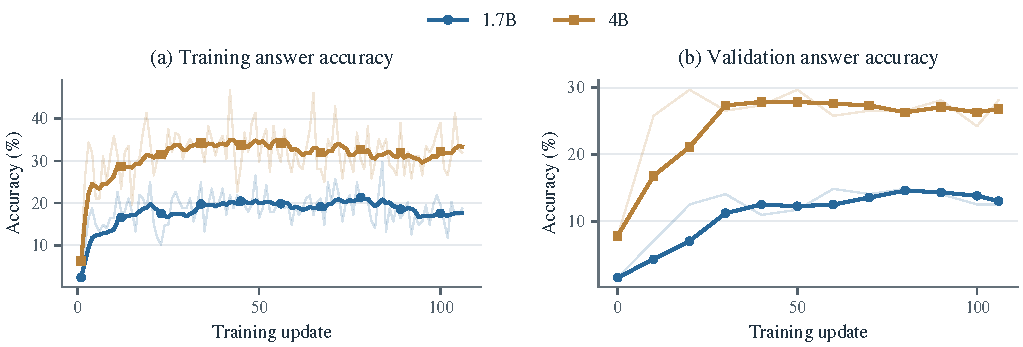
\includegraphics[width=\textwidth]{figures/accuracy_history.pdf}
\caption{FULL training and validation answer accuracy at both scales. Light curves retain raw observations; dark curves use trailing windows of ten updates for training and three observations for validation. Training responses are scored before optimization. Validation responses are freshly generated on the same excluded questions at each observation.}
\label{fig:accuracy_history}
\end{figure}
\begin{table}[!htbp]
\centering
\caption{Freshly generated answers on 128 validation questions excluded from training at each scale. Entries report FULL. Accuracy is percent; KL averages per-response token-mean losses.}
\label{tab:two_scale_validation}
\small
\setlength{\tabcolsep}{3pt}
\begin{tabular}{rrrrr}
\toprule
Step & 1.7B KL & 1.7B accuracy & 4B KL & 4B accuracy \\
\midrule
0 & 2.41500 & 1.56 & 1.97164 & 7.81 \\
10 & 0.17422 & 7.03 & 0.09756 & 25.78 \\
20 & 0.11939 & 12.50 & 0.07225 & 29.69 \\
30 & 0.10461 & 14.06 & 0.05850 & 26.56 \\
40 & 0.09494 & 10.94 & 0.05360 & 27.34 \\
50 & 0.08926 & 11.72 & 0.05054 & 29.69 \\
60 & 0.08781 & 14.84 & 0.04840 & 25.78 \\
70 & 0.08389 & 14.06 & 0.04799 & 26.56 \\
80 & 0.08461 & 14.84 & 0.04613 & 26.56 \\
90 & 0.08332 & 14.06 & 0.04441 & 28.13 \\
100 & 0.07893 & 12.50 & 0.04462 & 24.22 \\
106 & 0.07841 & 12.50 & 0.04450 & 28.13 \\
\bottomrule
\end{tabular}
\end{table}

\begin{table}[!htbp]
\centering
\caption{One-step validation transfer in paired-study FULL. Before/after losses use identical freshly generated validation prefixes. Actual and linear-predicted gains are multiplied by $10^3$; positive fraction uses gain $>10^{-6}$. Relative gain is $100G_V/(K_V(\theta)+10^{-12})$, with $K_V(\theta)$ evaluated on the same prefixes before the update. $c_g$ compares training and validation gradients.}
\label{tab:paired_transfer}
\small
\setlength{\tabcolsep}{3pt}
\begin{tabular}{lrrrrr}
\toprule
Before step  &  Actual  &  Predicted  &  Relative (\%)  &  Positive (\%)  &  $c_g$  \\
\midrule
0  &  1104.3261  &  9547.2064  &  45.735  &  100.00  &  0.7182  \\
10  &  12.5471  &  20.6128  &  7.202  &  100.00  &  0.9127  \\
20  &  2.2858  &  4.3104  &  1.915  &  86.72  &  0.6172  \\
30  &  0.7939  &  1.3757  &  0.759  &  70.31  &  0.3485  \\
40  &  0.5942  &  0.8148  &  0.626  &  71.88  &  0.2226  \\
50  &  0.4722  &  0.6193  &  0.529  &  67.19  &  0.2033  \\
60  &  0.4295  &  0.5707  &  0.489  &  68.75  &  0.1232  \\
70  &  0.2031  &  0.3146  &  0.242  &  57.03  &  0.1758  \\
80  &  -0.1346  &  0.1726  &  -0.159  &  46.09  &  0.2169  \\
90  &  0.5068  &  0.6088  &  0.608  &  67.97  &  0.2316  \\
100  &  0.1613  &  0.4004  &  0.204  &  63.28  &  0.2211  \\
\bottomrule
\end{tabular}
\end{table}

\begin{table}[!htbp]
\centering
\caption{4B. One-step validation transfer in paired-study FULL. Before/after losses use identical freshly generated validation prefixes. Actual and linear-predicted gains are multiplied by $10^3$; positive fraction uses gain $>10^{-6}$. Relative gain is $100G_V/(K_V(\theta)+10^{-12})$, with $K_V(\theta)$ evaluated on the same prefixes before the update. $c_g$ compares training and validation gradients.}
\label{tab:paired4b_transfer}
\small
\setlength{\tabcolsep}{3pt}
\begin{tabular}{lrrrrr}
\toprule
Before step  &  Actual  &  Predicted  &  Relative (\%)  &  Positive (\%)  &  $c_g$  \\
\midrule
0  &  966.1828  &  15190.3290  &  49.004  &  100.00  &  0.7868  \\
10  &  6.3733  &  12.3741  &  6.533  &  98.44  &  0.9220  \\
20  &  1.2939  &  2.3732  &  1.791  &  87.50  &  0.7011  \\
30  &  0.9536  &  1.6808  &  1.630  &  82.03  &  0.6321  \\
40  &  0.5023  &  0.8043  &  0.937  &  75.78  &  0.5518  \\
50  &  0.2109  &  0.4383  &  0.417  &  66.41  &  0.2588  \\
60  &  0.1734  &  0.3961  &  0.358  &  61.72  &  0.3278  \\
70  &  -0.0491  &  0.2486  &  -0.102  &  53.13  &  0.1267  \\
80  &  -0.0360  &  0.2738  &  -0.078  &  47.66  &  0.2230  \\
90  &  0.0017  &  0.3096  &  0.004  &  56.25  &  0.3463  \\
100  &  0.0319  &  0.2680  &  0.072  &  47.66  &  0.1927  \\
\bottomrule
\end{tabular}
\end{table}

\begin{figure}[!htbp]
\centering
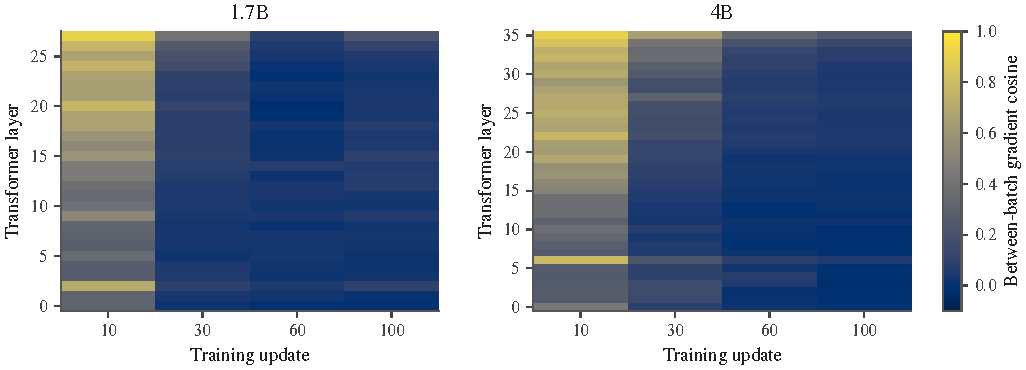
\includegraphics[width=\textwidth]{figures/two_scale_layers.pdf}
\caption{Layer-resolved FULL parameter-gradient agreement in both scales. Each heatmap compares four disjoint subsets at a fixed checkpoint; color is mean pairwise gradient cosine.}
\label{fig:two_scale_layers}
\end{figure}

\begin{table}[!htbp]
\centering
\caption{Adjacent-observation full-hidden gradient comparisons at both scales. Mean cosine retains signs; axis overlap is sign-invariant. Checkpoint and sampled batch both change across observations.}
\label{tab:two_scale_temporal}
\small
\setlength{\tabcolsep}{3pt}
\begin{tabular}{llrrrr}
\toprule
Model & Steps & Mean cosine & Axis-1 & Axes-4 & Axes-128 \\
\midrule
1.7B & 10--15 & -0.5526 & 0.9284 & 0.7837 & 0.7361 \\
1.7B & 15--20 & 0.1285 & 0.9840 & 0.9817 & 0.7701 \\
1.7B & 20--25 & -0.3374 & 0.9843 & 0.9809 & 0.7543 \\
1.7B & 25--30 & -0.2571 & 0.9680 & 0.8327 & 0.7536 \\
1.7B & 30--35 & -0.4686 & 0.9595 & 0.9857 & 0.7642 \\
1.7B & 35--40 & -0.1571 & 0.9887 & 0.9824 & 0.7592 \\
1.7B & 40--45 & -0.2392 & 0.9921 & 0.9543 & 0.7418 \\
1.7B & 45--50 & -0.1321 & 0.9890 & 0.9648 & 0.7452 \\
1.7B & 50--55 & -0.1673 & 0.9792 & 0.9630 & 0.7499 \\
1.7B & 55--60 & -0.0947 & 0.9797 & 0.9714 & 0.7305 \\
1.7B & 60--65 & -0.0592 & 0.9853 & 0.9829 & 0.7506 \\
1.7B & 65--70 & 0.0916 & 0.9837 & 0.9791 & 0.7667 \\
1.7B & 70--75 & 0.3569 & 0.9882 & 0.9862 & 0.7492 \\
1.7B & 75--80 & -0.1038 & 0.9894 & 0.9760 & 0.7448 \\
1.7B & 80--85 & -0.2730 & 0.9874 & 0.9737 & 0.7408 \\
1.7B & 85--90 & -0.2963 & 0.9870 & 0.9530 & 0.7326 \\
1.7B & 90--95 & -0.1807 & 0.9809 & 0.9797 & 0.7286 \\
1.7B & 95--100 & -0.5182 & 0.9843 & 0.9745 & 0.7417 \\
1.7B & 100--105 & -0.1978 & 0.9791 & 0.9712 & 0.7193 \\
1.7B & 105--106 & 0.4732 & 0.9846 & 0.9850 & 0.7500 \\
4B & 10--15 & -0.7348 & 0.7915 & 0.8909 & 0.7578 \\
4B & 15--20 & -0.1317 & 0.9848 & 0.9730 & 0.7447 \\
4B & 20--25 & -0.3701 & 0.9544 & 0.9833 & 0.7507 \\
4B & 25--30 & -0.4398 & 0.9877 & 0.9825 & 0.7248 \\
4B & 30--35 & -0.5330 & 0.9864 & 0.9881 & 0.7356 \\
4B & 35--40 & -0.3960 & 0.9907 & 0.9849 & 0.7428 \\
4B & 40--45 & -0.1945 & 0.9817 & 0.9852 & 0.7375 \\
4B & 45--50 & 0.0842 & 0.9914 & 0.9935 & 0.7534 \\
4B & 50--55 & 0.0132 & 0.9906 & 0.9818 & 0.7636 \\
4B & 55--60 & -0.0926 & 0.9909 & 0.9800 & 0.7584 \\
4B & 60--65 & -0.3121 & 0.9860 & 0.9893 & 0.7452 \\
4B & 65--70 & -0.1840 & 0.9842 & 0.9898 & 0.7471 \\
4B & 70--75 & 0.1847 & 0.9832 & 0.9465 & 0.7633 \\
4B & 75--80 & 0.2462 & 0.9804 & 0.9722 & 0.7444 \\
4B & 80--85 & -0.1207 & 0.9895 & 0.9882 & 0.7497 \\
4B & 85--90 & 0.0266 & 0.9873 & 0.9866 & 0.7433 \\
4B & 90--95 & 0.2088 & 0.9879 & 0.9260 & 0.7538 \\
4B & 95--100 & -0.0687 & 0.9857 & 0.9826 & 0.7588 \\
4B & 100--105 & 0.4022 & 0.9906 & 0.9381 & 0.7097 \\
4B & 105--106 & 0.4655 & 0.9826 & 0.9861 & 0.7261 \\
\bottomrule
\end{tabular}
\end{table}


\paragraph{Scale and directional factors of held-out gains.}
Table~\ref{tab:gain_factors} reports the factors in Equation~\ref{eq:gain_factors} at every recorded FULL observation. The product is checked against the stored linear prediction. Norms and cosines describe the actual parameter update and validation gradient; the residual compares the predicted and measured before/after KL change.
The actual parameter-step norm decreases substantially early in training and subsequently fluctuates at a lower level. The recorded learning rate remains $10^{-5}$ throughout both FULL runs. AdamW's gradient history and adaptive scaling remain part of the realized update. This norm measures the magnitude of the parameter displacement.
\begin{table}[!htbp]
\centering
\caption{Scale, direction, and finite-update effects in paired FULL. $c_\Delta=\cos(-g_V,\Delta\theta)$; $\widehat G_V=\|g_V\|\|\Delta\theta\|c_\Delta$; $R_V=G_V-\widehat G_V$. Only the last three columns are multiplied by $10^3$. Each comparison holds its validation responses fixed.}
\label{tab:gain_factors}
\small\setlength{\tabcolsep}{6pt}
\begin{tabular}{llrrrrrr}
\toprule
Model & Step & $\|g_V\|$ & $\|\Delta\theta\|$ & $c_\Delta$ & $10^3\widehat G_V$ & $10^3G_V$ & $10^3R_V$ \\
\midrule
\multirow{11}{*}{1.7B} & 0 & 166.52191 & 0.37070 & 0.15466 & 9547.20639 & 1104.32607 & -8442.88032 \\
 & 10 & 2.32557 & 0.17002 & 0.05213 & 20.61284 & 12.54712 & -8.06572 \\
 & 20 & 1.03405 & 0.13183 & 0.03162 & 4.31040 & 2.28581 & -2.02459 \\
 & 30 & 0.68095 & 0.10615 & 0.01903 & 1.37575 & 0.79386 & -0.58188 \\
 & 40 & 0.60345 & 0.09676 & 0.01396 & 0.81484 & 0.59421 & -0.22063 \\
 & 50 & 0.61362 & 0.09395 & 0.01074 & 0.61934 & 0.47220 & -0.14714 \\
 & 60 & 0.59056 & 0.08802 & 0.01098 & 0.57069 & 0.42954 & -0.14116 \\
 & 70 & 0.56834 & 0.08825 & 0.00627 & 0.31459 & 0.20313 & -0.11145 \\
 & 80 & 0.60931 & 0.08872 & 0.00319 & 0.17263 & -0.13456 & -0.30719 \\
 & 90 & 0.61603 & 0.08678 & 0.01139 & 0.60882 & 0.50681 & -0.10201 \\
 & 100 & 0.55462 & 0.08515 & 0.00848 & 0.40043 & 0.16135 & -0.23908 \\
\midrule
\multirow{11}{*}{4B} & 0 & 115.54819 & 0.59054 & 0.22262 & 15190.32898 & 966.18281 & -14224.14617 \\
 & 10 & 1.09561 & 0.21413 & 0.05275 & 12.37410 & 6.37332 & -6.00078 \\
 & 20 & 0.55525 & 0.15355 & 0.02784 & 2.37315 & 1.29395 & -1.07921 \\
 & 30 & 0.41294 & 0.13135 & 0.03099 & 1.68083 & 0.95356 & -0.72727 \\
 & 40 & 0.34231 & 0.12125 & 0.01938 & 0.80429 & 0.50230 & -0.30200 \\
 & 50 & 0.29828 & 0.11649 & 0.01261 & 0.43831 & 0.21086 & -0.22744 \\
 & 60 & 0.30162 & 0.11582 & 0.01134 & 0.39612 & 0.17338 & -0.22274 \\
 & 70 & 0.28557 & 0.13257 & 0.00657 & 0.24857 & -0.04907 & -0.29764 \\
 & 80 & 0.25265 & 0.12525 & 0.00865 & 0.27377 & -0.03596 & -0.30973 \\
 & 90 & 0.29183 & 0.12071 & 0.00879 & 0.30957 & 0.00165 & -0.30792 \\
 & 100 & 0.37719 & 0.11725 & 0.00606 & 0.26802 & 0.03191 & -0.23610 \\
\bottomrule
\end{tabular}
\medskip
\parbox{\linewidth}{\footnotesize From step 10 to 100, the 1.7B/4B norm ratios are $0.2385/0.3443$ for $g_V$ and $0.5008/0.5476$ for $\Delta\theta$; alignment ratios are $0.1626/0.1149$. The linear-gain ratios are $0.01943/0.02166$. At step 100, actual/predicted gain is $0.4029/0.1191$. These multiplicative ratios describe measured changes; they do not independently identify causal contributions.}
\end{table}


\FloatBarrier
\subsection{Matched Diagnostics and Subsequent Held-Out Gains}
\label{app:matched_diagnostics}
Table~\ref{tab:joint_checkpoint_audit} aligns the available diagnostics at the four checkpoints with complete cross-subset measurements in each model. Gradient statistics use four disjoint subsets evaluated at the checkpoint parameters. For subset $b$, let $g_h$ be a token-level gradient in the full hidden space. The reported coherence is
\begin{equation}
 C_h=\frac14\sum_{b=1}^4
 \frac{\|\mathbb E_b[g_h]\|^2}{\mathbb E_b[\|g_h\|^2]}.
\end{equation}
Table~\ref{tab:space_coherence} gives the corresponding projected-space measurements. The mean parameter-gradient norm averages the four subset norms; the pairwise cosines and covariance overlap average the six subset pairs. Each row pairs these checkpoint diagnostics with the measured effect of the next actual training update on validation responses held fixed across that update. Training-loss summaries use only batches completed by the checkpoint.

This alignment makes the concurrent changes in loss, gradient scale, agreement, geometry, and actual gain directly inspectable. Coherence falls as the squared mean gradient becomes smaller relative to its second moment. The matched observations comprise four checkpoints from one FULL trajectory per scale. The linear prediction in Table~\ref{tab:gain_factors} uses the validation gradient and realized update to describe that same step.

\begin{table}[!htbp]
\centering
\caption{Matched checkpoint observations in paired FULL. Panels share the same rows. $K_t$ is the last training-batch KL and $s_t=(K_{t-5}-K_t)/5$ is its preceding five-update decline per update; the batches differ. $\overline{\|g_\theta\|}$ averages parameter-gradient norms across four disjoint subsets. $C_h$ averages full-hidden token coherence over those subsets. $c_h$ and $c_\theta$ average six mean-hidden and parameter-gradient pairwise cosines; $O_4$ averages centered top-4 covariance overlap. $E_U$ is cumulative displacement coverage. $G_V$ is the actual validation KL reduction from one training update starting at that checkpoint; its relative value uses pre-update validation KL. These are aligned descriptive observations.}
\label{tab:joint_checkpoint_audit}
\small\setlength{\tabcolsep}{7pt}
\textbf{(a) Training loss, gradient scale, and agreement}\par\smallskip
\begin{tabular}{llrrrrrr}
\toprule
Model & Step & $K_t$ & $10^3s_t$ & $\overline{\|g_\theta\|}$ & $10^3C_h$ & $c_h$ & $c_\theta$ \\
\midrule
\multirow{4}{*}{1.7B} & 10 & 0.18739 & 24.1974 & 2.37265 & 0.79223 & 0.8977 & 0.7325 \\
 & 30 & 0.09843 & 1.3070 & 1.09367 & 0.07463 & 0.3874 & 0.1100 \\
 & 60 & 0.08981 & -0.4135 & 1.00090 & 0.04696 & 0.0944 & 0.0396 \\
 & 100 & 0.07552 & 0.4286 & 0.96489 & 0.05441 & 0.2323 & 0.0828 \\
\midrule
\multirow{4}{*}{4B} & 10 & 0.10250 & 15.3189 & 1.14362 & 0.39586 & 0.8891 & 0.7696 \\
 & 30 & 0.06374 & -0.0057 & 0.55616 & 0.13150 & 0.6550 & 0.3346 \\
 & 60 & 0.05059 & 0.3247 & 0.47274 & 0.05913 & 0.3434 & 0.1029 \\
 & 100 & 0.04314 & -0.2902 & 0.51272 & 0.05805 & 0.2460 & 0.0596 \\
\bottomrule
\end{tabular}
\par\medskip
\textbf{(b) Geometry and the subsequent actual validation gain}\par\smallskip
\begin{tabular}{llrrrrr}
\toprule
Model & Step & $O_4$ & $E_U$ (\%) & $K_V$ before & $10^3G_V$ & Relative gain (\%) \\
\midrule
\multirow{4}{*}{1.7B} & 10 & 0.9528 & 85.66 & 0.17422 & 12.54712 & 7.202 \\
 & 30 & 0.8411 & 86.48 & 0.10461 & 0.79386 & 0.759 \\
 & 60 & 0.7881 & 87.00 & 0.08781 & 0.42954 & 0.489 \\
 & 100 & 0.8895 & 87.28 & 0.07893 & 0.16135 & 0.204 \\
\midrule
\multirow{4}{*}{4B} & 10 & 0.9700 & 80.50 & 0.09756 & 6.37332 & 6.533 \\
 & 30 & 0.9553 & 80.09 & 0.05850 & 0.95356 & 1.630 \\
 & 60 & 0.8917 & 79.46 & 0.04840 & 0.17338 & 0.358 \\
 & 100 & 0.9471 & 79.06 & 0.04462 & 0.03191 & 0.072 \\
\bottomrule
\end{tabular}
\end{table}

\clearpage
\makeatletter
\setlength{\@fptop}{0pt}
\makeatother
\subsection{Parameter-Space Update Dynamics}
\label{app:parameter_dynamics}
This section consolidates the parameter-level measurements from the paired FULL trajectories: realized update magnitude, its distribution across parameter groups and layers, update direction, and the spectrum of sampled parameter gradients. All measurements refer to the same two training runs used in the main analysis. Tables~\ref{tab:parameter_update_groups}--\ref{tab:parameter_gradient_spectrum} report the numerical results.

\paragraph{Measured objects and parameter groups.}
For an observed training step starting at checkpoint $t$, we capture the parameters before and after the optimizer step and form $\Delta\theta_t=\theta_{t+1}-\theta_t$. For group $S$, its update magnitude and squared-norm share are
\begin{equation}
 m_{S,t}=\|\Delta\theta_{S,t}\|_2,\qquad
 f_{S,t}=\frac{\|\Delta\theta_{S,t}\|_2^2}{\|\Delta\theta_t\|_2^2}.
\end{equation}
The diagnostics sum exact inner products over distributed parameter shards. Both models tie their input embeddings and output weights, so these coordinates form one shared embedding/head group. Backbone denotes the remaining parameters and includes Transformer blocks and the final normalization parameters. Layer groups index individual Transformer blocks. The backbone and shared group partition the full parameter vector; layer groups are subsets of the backbone. Norms are absolute and unnormalized by parameter count. The recorded gradient $g_T$ is captured at the optimizer boundary, while the independent cross-subset gradients are computed for their respective diagnostic batches.

\paragraph{How much do parameters move?}
The realized parameter-step magnitude falls sharply during early training, followed by smaller fluctuations (Table~\ref{tab:parameter_update_groups}). The late 4B trajectory includes a temporary rebound. All recorded learning rates are constant, so this trend occurs with a fixed nominal step size. AdamW's moments, adaptive scaling, and the current gradient jointly determine the actual displacement. Training-gradient norms also decrease between the early and late observations, while the optimizer step retains its own temporal profile. The complete validation-gradient and update-norm series in Table~\ref{tab:gain_factors} connects these parameter changes to the measured held-out gains.

\paragraph{Where do updates occur?}
Most squared update magnitude lies in the backbone at every recorded diagnostic. The shared embedding/head contributes a smaller fraction, whose relative share increases between the selected early and late observations (Table~\ref{tab:parameter_update_groups}). Tables~\ref{tab:parameter_layers_17} and~\ref{tab:parameter_layers_4b} resolve every Transformer block at the checkpoints with complete cross-subset diagnostics. Every layer has a nonzero aggregate update norm, and every layer's norm is smaller at the last selected checkpoint than at the first. The largest-update layers change over training, so the spatial profile also changes. These group-level measurements locate update magnitude within the network. Group sizes affect their absolute norms, and a nonzero layer norm permits many unchanged coordinates inside that layer.

\paragraph{How do update directions change?}
We distinguish agreement across training subsets, agreement between training and validation gradients, and the direction of the realized optimizer step. Cross-subset parameter-gradient cosines weaken across the network (Tables~\ref{tab:parameter_layers_17} and~\ref{tab:parameter_layers_4b}; Figure~\ref{fig:two_scale_layers}). At the full-model level, most measured pairs remain nonnegative (Table~\ref{tab:two_scale_batch}). The cosine $c_{T,V}=\cos(g_T,g_V)$ compares the current training and validation gradients. The cosine $c_{T,\Delta}=\cos(-g_T,\Delta\theta)$ compares the actual step with current training descent; its early-to-late increase in both models coexists with the decrease in update alignment to validation descent reported in Table~\ref{tab:gain_factors}. In these observations, AdamW follows current training descent more closely while providing less improvement on validation responses.

\begin{table}[!htbp]
\centering
\caption{Parameter-scale measurements at all FULL update diagnostics. $g_T$ is the recorded training gradient at the optimizer boundary; $c_{T,\Delta}=\cos(-g_T,\Delta\theta)$ and $c_{T,V}=\cos(g_T,g_V)$. BB denotes backbone; SH denotes the shared embedding/output matrix. SH share is its fraction of the full squared update norm. Shared weights are counted once. Norms are absolute, with no parameter-count normalization.}
\label{tab:parameter_update_groups}
\small\setlength{\tabcolsep}{5pt}
\begin{tabular}{llrrrrrrr}
\toprule
Model & Step & $\|g_T\|$ & $\|\Delta\theta\|$ & BB norm & SH norm & SH (\%) & $c_{T,\Delta}$ & $c_{T,V}$ \\
\midrule
\multirow{11}{*}{1.7B} & 0 & 9.73485 & 0.37070 & 0.36472 & 0.06631 & 3.19944 & 0.12773 & 0.71820 \\
 & 10 & 2.11610 & 0.17002 & 0.16862 & 0.02177 & 1.63917 & 0.07628 & 0.91269 \\
 & 20 & 0.89307 & 0.13183 & 0.13035 & 0.01965 & 2.22180 & 0.08775 & 0.61717 \\
 & 30 & 0.63031 & 0.10615 & 0.10464 & 0.01784 & 2.82560 & 0.12169 & 0.34850 \\
 & 40 & 0.53691 & 0.09676 & 0.09530 & 0.01673 & 2.98910 & 0.12327 & 0.22256 \\
 & 50 & 0.65648 & 0.09395 & 0.09253 & 0.01629 & 3.00666 & 0.14533 & 0.20330 \\
 & 60 & 0.53830 & 0.08802 & 0.08650 & 0.01632 & 3.43806 & 0.14009 & 0.12318 \\
 & 70 & 0.56296 & 0.08825 & 0.08693 & 0.01517 & 2.95478 & 0.13882 & 0.17576 \\
 & 80 & 0.55486 & 0.08872 & 0.08735 & 0.01557 & 3.07801 & 0.12963 & 0.21693 \\
 & 90 & 0.61441 & 0.08678 & 0.08542 & 0.01531 & 3.11431 & 0.14288 & 0.23159 \\
 & 100 & 0.54322 & 0.08515 & 0.08378 & 0.01522 & 3.19642 & 0.12356 & 0.22113 \\
\midrule
\multirow{11}{*}{4B} & 0 & 5.56719 & 0.59054 & 0.58431 & 0.08557 & 2.09971 & 0.19317 & 0.78677 \\
 & 10 & 1.04053 & 0.21413 & 0.21254 & 0.02605 & 1.48024 & 0.08325 & 0.92204 \\
 & 20 & 0.50576 & 0.15355 & 0.15207 & 0.02126 & 1.91705 & 0.10195 & 0.70109 \\
 & 30 & 0.39394 & 0.13135 & 0.12997 & 0.01900 & 2.09256 & 0.11647 & 0.63208 \\
 & 40 & 0.32492 & 0.12125 & 0.11997 & 0.01758 & 2.10218 & 0.12731 & 0.55178 \\
 & 50 & 0.28348 & 0.11649 & 0.11517 & 0.01744 & 2.24244 & 0.18620 & 0.25881 \\
 & 60 & 0.27415 & 0.11582 & 0.11454 & 0.01718 & 2.19999 & 0.16674 & 0.32781 \\
 & 70 & 0.46498 & 0.13257 & 0.13152 & 0.01668 & 1.58328 & 0.28753 & 0.12675 \\
 & 80 & 0.25080 & 0.12525 & 0.12410 & 0.01690 & 1.82166 & 0.15812 & 0.22303 \\
 & 90 & 0.29867 & 0.12071 & 0.11958 & 0.01648 & 1.86415 & 0.18945 & 0.34634 \\
 & 100 & 0.27971 & 0.11725 & 0.11604 & 0.01679 & 2.05109 & 0.20012 & 0.19271 \\
\bottomrule
\end{tabular}
\end{table}

\begin{table}[!htbp]
\centering
\caption{1.7B FULL: every Transformer layer at the four checkpoints with complete cross-batch measurements. Update columns are $10^3\|\Delta\theta_\ell\|$; drop is the percentage decrease from step 10 to 100. Share uses $\|\Delta\theta_\ell\|^2/\|\Delta\theta\|^2$ at step 100. $g_{T,\ell}$ is the recorded training gradient; $c_{B,\ell}$ averages six cross-subset parameter-gradient cosines. Layer indices start at zero. These absolute group norms reflect both coordinate count and update magnitude.}
\label{tab:parameter_layers_17}
\fontsize{8.5}{10.5}\selectfont\setlength{\tabcolsep}{4pt}
\begin{tabular}{rrrrrrrrrrr}
\toprule
Layer & $\Delta_{10}$ & $\Delta_{30}$ & $\Delta_{60}$ & $\Delta_{100}$ & Drop (\%) & Share (\%) & $g_{T,10}$ & $g_{T,100}$ & $c_{B,10}$ & $c_{B,100}$ \\
\midrule
0 & 28.5392 & 18.2978 & 15.0611 & 14.7544 & 48.3011 & 3.0026 & 0.0714 & 0.0387 & 0.3097 & 0.0042 \\
1 & 28.9061 & 18.1933 & 15.1164 & 14.6661 & 49.2629 & 2.9668 & 0.0836 & 0.0447 & 0.3087 & 0.0078 \\
2 & 28.4473 & 18.5095 & 15.3807 & 15.3133 & 46.1696 & 3.2344 & 1.2392 & 0.3580 & 0.7117 & 0.1003 \\
3 & 28.4521 & 18.7173 & 15.5263 & 15.4457 & 45.7133 & 3.2906 & 0.0924 & 0.0549 & 0.2669 & 0.0288 \\
4 & 28.7060 & 18.8239 & 15.6663 & 15.7265 & 45.2152 & 3.4113 & 0.1051 & 0.0578 & 0.2729 & 0.0144 \\
5 & 28.9928 & 18.9546 & 15.9783 & 15.9867 & 44.8596 & 3.5251 & 0.1108 & 0.0568 & 0.3533 & 0.0175 \\
6 & 29.0030 & 19.1382 & 16.2311 & 16.1744 & 44.2321 & 3.6084 & 0.1105 & 0.0635 & 0.2777 & 0.0280 \\
7 & 28.8404 & 19.1738 & 16.4154 & 16.1713 & 43.9284 & 3.6070 & 0.1243 & 0.0695 & 0.3021 & 0.0309 \\
8 & 29.1807 & 19.2442 & 16.4363 & 16.2509 & 44.3094 & 3.6426 & 0.1326 & 0.0712 & 0.3196 & 0.0267 \\
9 & 29.9477 & 19.4434 & 16.4094 & 16.1779 & 45.9794 & 3.6099 & 0.2166 & 0.0906 & 0.5185 & 0.0558 \\
10 & 30.6678 & 19.6503 & 16.5182 & 16.3226 & 46.7761 & 3.6748 & 0.1775 & 0.0829 & 0.3840 & 0.0256 \\
11 & 30.8244 & 19.7777 & 16.6616 & 16.4816 & 46.5304 & 3.7467 & 0.2141 & 0.1097 & 0.3401 & 0.0300 \\
12 & 31.3510 & 19.9227 & 16.6729 & 16.3904 & 47.7197 & 3.7054 & 0.1979 & 0.1012 & 0.3763 & 0.0694 \\
13 & 31.9229 & 19.9186 & 16.5411 & 16.1926 & 49.2761 & 3.6165 & 0.2384 & 0.1046 & 0.4493 & 0.0669 \\
14 & 32.5604 & 19.9967 & 16.6029 & 16.2157 & 50.1980 & 3.6268 & 0.2486 & 0.1042 & 0.4513 & 0.0616 \\
15 & 33.7831 & 20.0909 & 16.6006 & 16.1607 & 52.1634 & 3.6022 & 0.3007 & 0.1119 & 0.5834 & 0.0955 \\
16 & 34.2905 & 20.1193 & 16.6496 & 16.2528 & 52.6025 & 3.6434 & 0.2528 & 0.0976 & 0.5337 & 0.0513 \\
17 & 35.2561 & 20.4515 & 16.5557 & 15.9998 & 54.6183 & 3.5309 & 0.2741 & 0.0942 & 0.5916 & 0.0450 \\
18 & 35.4101 & 20.5374 & 16.3918 & 15.8007 & 55.3780 & 3.4435 & 0.2571 & 0.0788 & 0.6702 & 0.0695 \\
19 & 35.7539 & 20.6354 & 16.4086 & 15.8307 & 55.7232 & 3.4566 & 0.1996 & 0.0595 & 0.6634 & 0.0414 \\
20 & 35.1994 & 20.3489 & 16.6649 & 16.0176 & 54.4948 & 3.5387 & 0.2465 & 0.0639 & 0.7699 & 0.0460 \\
21 & 34.0487 & 20.5502 & 17.2071 & 16.1270 & 52.6356 & 3.5872 & 0.1376 & 0.0441 & 0.6468 & 0.0396 \\
22 & 33.2680 & 20.8258 & 17.4399 & 16.5505 & 50.2510 & 3.7781 & 0.1194 & 0.0367 & 0.6464 & 0.0367 \\
23 & 32.4074 & 20.6600 & 17.6203 & 16.5597 & 48.9013 & 3.7823 & 0.1025 & 0.0309 & 0.6612 & 0.0236 \\
24 & 32.3908 & 20.7181 & 17.1187 & 16.2198 & 49.9246 & 3.6287 & 0.1199 & 0.0283 & 0.7469 & 0.0379 \\
25 & 33.9878 & 20.2538 & 15.9578 & 14.8106 & 56.4239 & 3.0255 & 0.0958 & 0.0252 & 0.6699 & 0.0614 \\
26 & 34.2586 & 20.5238 & 16.0691 & 14.4848 & 57.7192 & 2.8939 & 0.1588 & 0.0314 & 0.7685 & 0.1129 \\
27 & 33.1643 & 19.7945 & 15.4445 & 13.7918 & 58.4136 & 2.6236 & 1.0751 & 0.1155 & 0.9034 & 0.2205 \\
\bottomrule
\end{tabular}
\end{table}

\begin{table}[!htbp]
\centering
\caption{4B FULL: every Transformer layer at the four checkpoints with complete cross-batch measurements. Update columns are $10^3\|\Delta\theta_\ell\|$; drop is the percentage decrease from step 10 to 100. Share uses $\|\Delta\theta_\ell\|^2/\|\Delta\theta\|^2$ at step 100. $g_{T,\ell}$ is the recorded training gradient; $c_{B,\ell}$ averages six cross-subset parameter-gradient cosines. Layer indices start at zero. These absolute group norms reflect both coordinate count and update magnitude.}
\label{tab:parameter_layers_4b}
\fontsize{8.5}{10.5}\selectfont\setlength{\tabcolsep}{4pt}
\begin{tabular}{rrrrrrrrrrr}
\toprule
Layer & $\Delta_{10}$ & $\Delta_{30}$ & $\Delta_{60}$ & $\Delta_{100}$ & Drop (\%) & Share (\%) & $g_{T,10}$ & $g_{T,100}$ & $c_{B,10}$ & $c_{B,100}$ \\
\midrule
0 & 29.1959 & 17.7646 & 14.8206 & 15.8020 & 45.8760 & 1.8163 & 0.0410 & 0.0124 & 0.4312 & -0.0011 \\
1 & 26.0534 & 14.6271 & 12.4307 & 12.9267 & 50.3839 & 1.2154 & 0.0434 & 0.0167 & 0.2577 & -0.0081 \\
2 & 26.2831 & 15.3775 & 12.9734 & 13.4903 & 48.6730 & 1.3237 & 0.0453 & 0.0179 & 0.2669 & -0.0078 \\
3 & 28.5683 & 16.9525 & 14.5230 & 15.0643 & 47.2691 & 1.6507 & 0.0481 & 0.0196 & 0.2493 & -0.0241 \\
4 & 30.1748 & 19.8425 & 16.7710 & 17.5717 & 41.7671 & 2.2459 & 0.0508 & 0.0236 & 0.2382 & 0.0025 \\
5 & 31.3474 & 20.5939 & 17.6927 & 19.0343 & 39.2794 & 2.6353 & 0.0449 & 0.0251 & 0.2619 & -0.0030 \\
6 & 32.1227 & 20.8518 & 18.9521 & 20.3313 & 36.7073 & 3.0067 & 0.4413 & 0.1194 & 0.7834 & 0.0583 \\
7 & 32.1088 & 21.0028 & 19.5087 & 21.0723 & 34.3723 & 3.2298 & 0.0561 & 0.0344 & 0.2465 & -0.0056 \\
8 & 32.1888 & 21.0963 & 19.6572 & 20.5003 & 36.3123 & 3.0569 & 0.0465 & 0.0270 & 0.2813 & -0.0068 \\
9 & 32.2965 & 21.3852 & 19.9176 & 20.2892 & 37.1782 & 2.9943 & 0.0545 & 0.0324 & 0.3304 & -0.0132 \\
10 & 33.3425 & 21.8095 & 20.2846 & 20.3208 & 39.0544 & 3.0036 & 0.0638 & 0.0372 & 0.3732 & -0.0058 \\
11 & 34.1900 & 22.0193 & 20.6096 & 20.7065 & 39.4370 & 3.1187 & 0.0574 & 0.0416 & 0.3003 & 0.0170 \\
12 & 34.5956 & 22.1484 & 20.7865 & 20.7253 & 40.0928 & 3.1244 & 0.0699 & 0.0443 & 0.3725 & 0.0068 \\
13 & 34.9641 & 22.0929 & 20.8842 & 21.1180 & 39.6009 & 3.2439 & 0.0741 & 0.0484 & 0.3741 & 0.0139 \\
14 & 35.3915 & 22.0963 & 20.9513 & 20.8901 & 40.9743 & 3.1742 & 0.0825 & 0.0531 & 0.3752 & 0.0200 \\
15 & 35.7551 & 22.0762 & 21.0458 & 20.8433 & 41.7055 & 3.1600 & 0.1069 & 0.0571 & 0.4993 & 0.0148 \\
16 & 36.3139 & 22.3704 & 21.2301 & 20.9569 & 42.2895 & 3.1946 & 0.1086 & 0.0541 & 0.5251 & 0.0133 \\
17 & 37.1066 & 22.5181 & 21.1737 & 20.6448 & 44.3634 & 3.1001 & 0.1221 & 0.0549 & 0.5893 & 0.0117 \\
18 & 37.5812 & 23.0850 & 21.1731 & 20.7903 & 44.6789 & 3.1440 & 0.1252 & 0.0594 & 0.5691 & 0.0219 \\
19 & 37.6048 & 23.0392 & 20.9349 & 21.0490 & 44.0259 & 3.2227 & 0.1536 & 0.0598 & 0.6918 & 0.0229 \\
20 & 37.5979 & 22.9987 & 21.0228 & 21.3339 & 43.2579 & 3.3105 & 0.1274 & 0.0543 & 0.6332 & 0.0350 \\
21 & 37.7973 & 22.4432 & 20.3992 & 20.3764 & 46.0903 & 3.0200 & 0.1406 & 0.0548 & 0.6457 & 0.0484 \\
22 & 38.3860 & 22.5657 & 20.1215 & 19.9699 & 47.9761 & 2.9008 & 0.1629 & 0.0457 & 0.7732 & 0.0496 \\
23 & 38.5303 & 23.2800 & 20.3606 & 20.4353 & 46.9632 & 3.0375 & 0.1155 & 0.0423 & 0.6655 & 0.0430 \\
24 & 38.0280 & 23.0559 & 19.6875 & 20.1210 & 47.0889 & 2.9448 & 0.1044 & 0.0352 & 0.6934 & 0.0392 \\
25 & 38.3911 & 23.1168 & 19.3505 & 19.6458 & 48.8274 & 2.8074 & 0.0947 & 0.0309 & 0.7291 & 0.0417 \\
26 & 38.2576 & 23.1652 & 19.6860 & 19.9390 & 47.8824 & 2.8918 & 0.0798 & 0.0266 & 0.7004 & 0.0603 \\
27 & 38.4101 & 23.1590 & 19.3443 & 19.5005 & 49.2306 & 2.7660 & 0.0753 & 0.0254 & 0.6966 & 0.0525 \\
28 & 38.3554 & 23.3121 & 19.6318 & 19.7896 & 48.4047 & 2.8486 & 0.0733 & 0.0270 & 0.6636 & 0.0435 \\
29 & 37.2217 & 23.0867 & 19.8370 & 19.8611 & 46.6411 & 2.8692 & 0.0517 & 0.0214 & 0.6063 & 0.0443 \\
30 & 38.0454 & 23.4172 & 19.9229 & 19.8458 & 47.8366 & 2.8648 & 0.0663 & 0.0213 & 0.7097 & 0.0399 \\
31 & 37.7351 & 23.1384 & 19.5712 & 19.8945 & 47.2785 & 2.8789 & 0.0540 & 0.0204 & 0.6776 & 0.0477 \\
32 & 38.5044 & 22.6042 & 18.1209 & 18.4872 & 51.9867 & 2.4860 & 0.0676 & 0.0193 & 0.7736 & 0.0811 \\
33 & 38.4917 & 22.4132 & 17.1133 & 16.8834 & 56.1376 & 2.0734 & 0.0629 & 0.0183 & 0.7424 & 0.0849 \\
34 & 38.9424 & 21.4482 & 16.2778 & 16.1506 & 58.5270 & 1.8973 & 0.1218 & 0.0242 & 0.8358 & 0.1393 \\
35 & 38.4449 & 20.0076 & 15.1643 & 15.2451 & 60.3457 & 1.6905 & 0.5082 & 0.0778 & 0.8999 & 0.2473 \\
\bottomrule
\end{tabular}
\end{table}


\FloatBarrier
\paragraph{Spectrum of sampled parameter gradients.}
At each complete cross-subset checkpoint, let $g_1,\ldots,g_4\in\mathbb R^P$ be the four parameter gradients and $G=[g_1,\ldots,g_4]$. The saved Gram matrix $K=G^\top G$ gives the nonzero eigenvalues of $GG^\top$ exactly. With $p_i=\lambda_i(K)/\operatorname{tr}K$, we report its participation dimension $r_{\mathrm{PR}}=(\sum_i p_i^2)^{-1}$ and all four energy shares in Table~\ref{tab:parameter_gradient_spectrum}. We also repeat the calculation on $D^{-1/2}KD^{-1/2}$, where $D=\operatorname{diag}(K)$, to compare unit-normalized gradients.

The first spectral component loses share and the participation dimension increases between the early and late checkpoints at both scales. The increase persists after individual gradient normalization, supporting a broader spread of directions within the sampled panel. Together with the smaller parameter-step norms, these measurements show that update magnitude can shrink while sampled gradient directions become less concentrated. The panel contains four vectors and has an effective dimension bounded by four, describing variation across those sampled gradients.

\begin{table}[!htbp]
\centering
\caption{Spectrum of four sampled parameter gradients in FULL, recomputed from their exact $4\times4$ Gram matrix. Columns $p_1$--$p_4$ are descending eigenvalue energy shares. $r_{\mathrm{PR}}=1/\sum_i p_i^2$ measures concentration across these four vectors. The unit-norm column repeats the calculation after normalizing each gradient, reducing sensitivity to differences in gradient magnitude. Both dimensions are bounded by four and describe this sampled gradient panel.}
\label{tab:parameter_gradient_spectrum}
\small\setlength{\tabcolsep}{5pt}
\begin{tabular}{llrrrrrr}
\toprule
Model & Step & $p_1$ (\%) & $p_2$ (\%) & $p_3$ (\%) & $p_4$ (\%) & $r_{\mathrm{PR}}$ & Unit-norm $r_{\mathrm{PR}}$ \\
\midrule
\multirow{4}{*}{1.7B} & 10 & 79.7996 & 8.9037 & 6.4452 & 4.8515 & 1.5355 & 1.5310 \\
 & 30 & 33.6677 & 26.1973 & 20.9268 & 19.2082 & 3.8071 & 3.8473 \\
 & 60 & 32.8627 & 24.5767 & 22.7589 & 19.8017 & 3.8550 & 3.9724 \\
 & 100 & 33.1277 & 25.8583 & 21.7333 & 19.2807 & 3.8312 & 3.9063 \\
\midrule
\multirow{4}{*}{4B} & 10 & 82.7199 & 6.3077 & 6.0838 & 4.8886 & 1.4402 & 1.4401 \\
 & 30 & 50.1693 & 20.6059 & 16.0582 & 13.1666 & 2.9649 & 2.9891 \\
 & 60 & 36.5036 & 25.8851 & 19.4727 & 18.1386 & 3.6890 & 3.8682 \\
 & 100 & 40.2558 & 25.3514 & 18.0428 & 16.3500 & 3.5013 & 3.9491 \\
\bottomrule
\end{tabular}
\end{table}


